
\section{Cơ sở lý thuyết về phần cứng và cảm biến}

% Introducing the role of hardware in the system
Phần cứng là nền tảng vật lý của hệ thống phát hiện té ngã, chịu trách nhiệm thu thập, xử lý sơ bộ và truyền dữ liệu. Việc lựa chọn phần cứng phù hợp đảm bảo hiệu suất, độ tin cậy, tối ưu hóa chi phí và năng lượng. Các thành phần chính bao gồm hệ thống nhúng, cảm biến, thiết bị giám sát hình ảnh và hệ thống truyền thông, tích hợp để tạo thành hệ thống giám sát toàn diện.

% Subsection for embedded systems and sensors
\subsection{Hệ thống nhúng và cảm biến}

Hệ thống nhúng đóng vai trò trung tâm trong việc thu thập và xử lý dữ liệu tại biên, đặc biệt với các thiết bị đeo được hoặc cảm biến cố định.

\subsubsection{Vi điều khiển (Microcontroller)}
Vi điều khiển là bộ phận xử lý chính, đảm bảo khả năng tính toán và kết nối. Trong các dự án IoT, các vi điều khiển như Arduino, STM32 và ESP32 được sử dụng rộng rãi. Đối với hệ thống phát hiện té ngã, \textbf{ESP32} được ưu tiên nhờ kiến trúc hai nhân (Tensilica Xtensa LX6, 240 MHz), tích hợp Wi-Fi (802.11 b/g/n) và Bluetooth (v4.2/BLE), bộ nhớ flash 4--16 MB và hỗ trợ giao tiếp I2C/SPI \cite{esp32datasheet2023}. ESP32 xử lý dữ liệu cảm biến thời gian thực, truyền dữ liệu không dây và duy trì hiệu suất với mức tiêu thụ năng lượng thấp (5 mA ở chế độ chờ) \cite{iotproject2024}. So với Arduino Uno (16 MHz, không có Wi-Fi tích hợp), ESP32 vượt trội về hiệu năng và kết nối, phù hợp với giám sát liên tục và truyền thông từ xa.

\begin{figure}[ht]
    \centering
    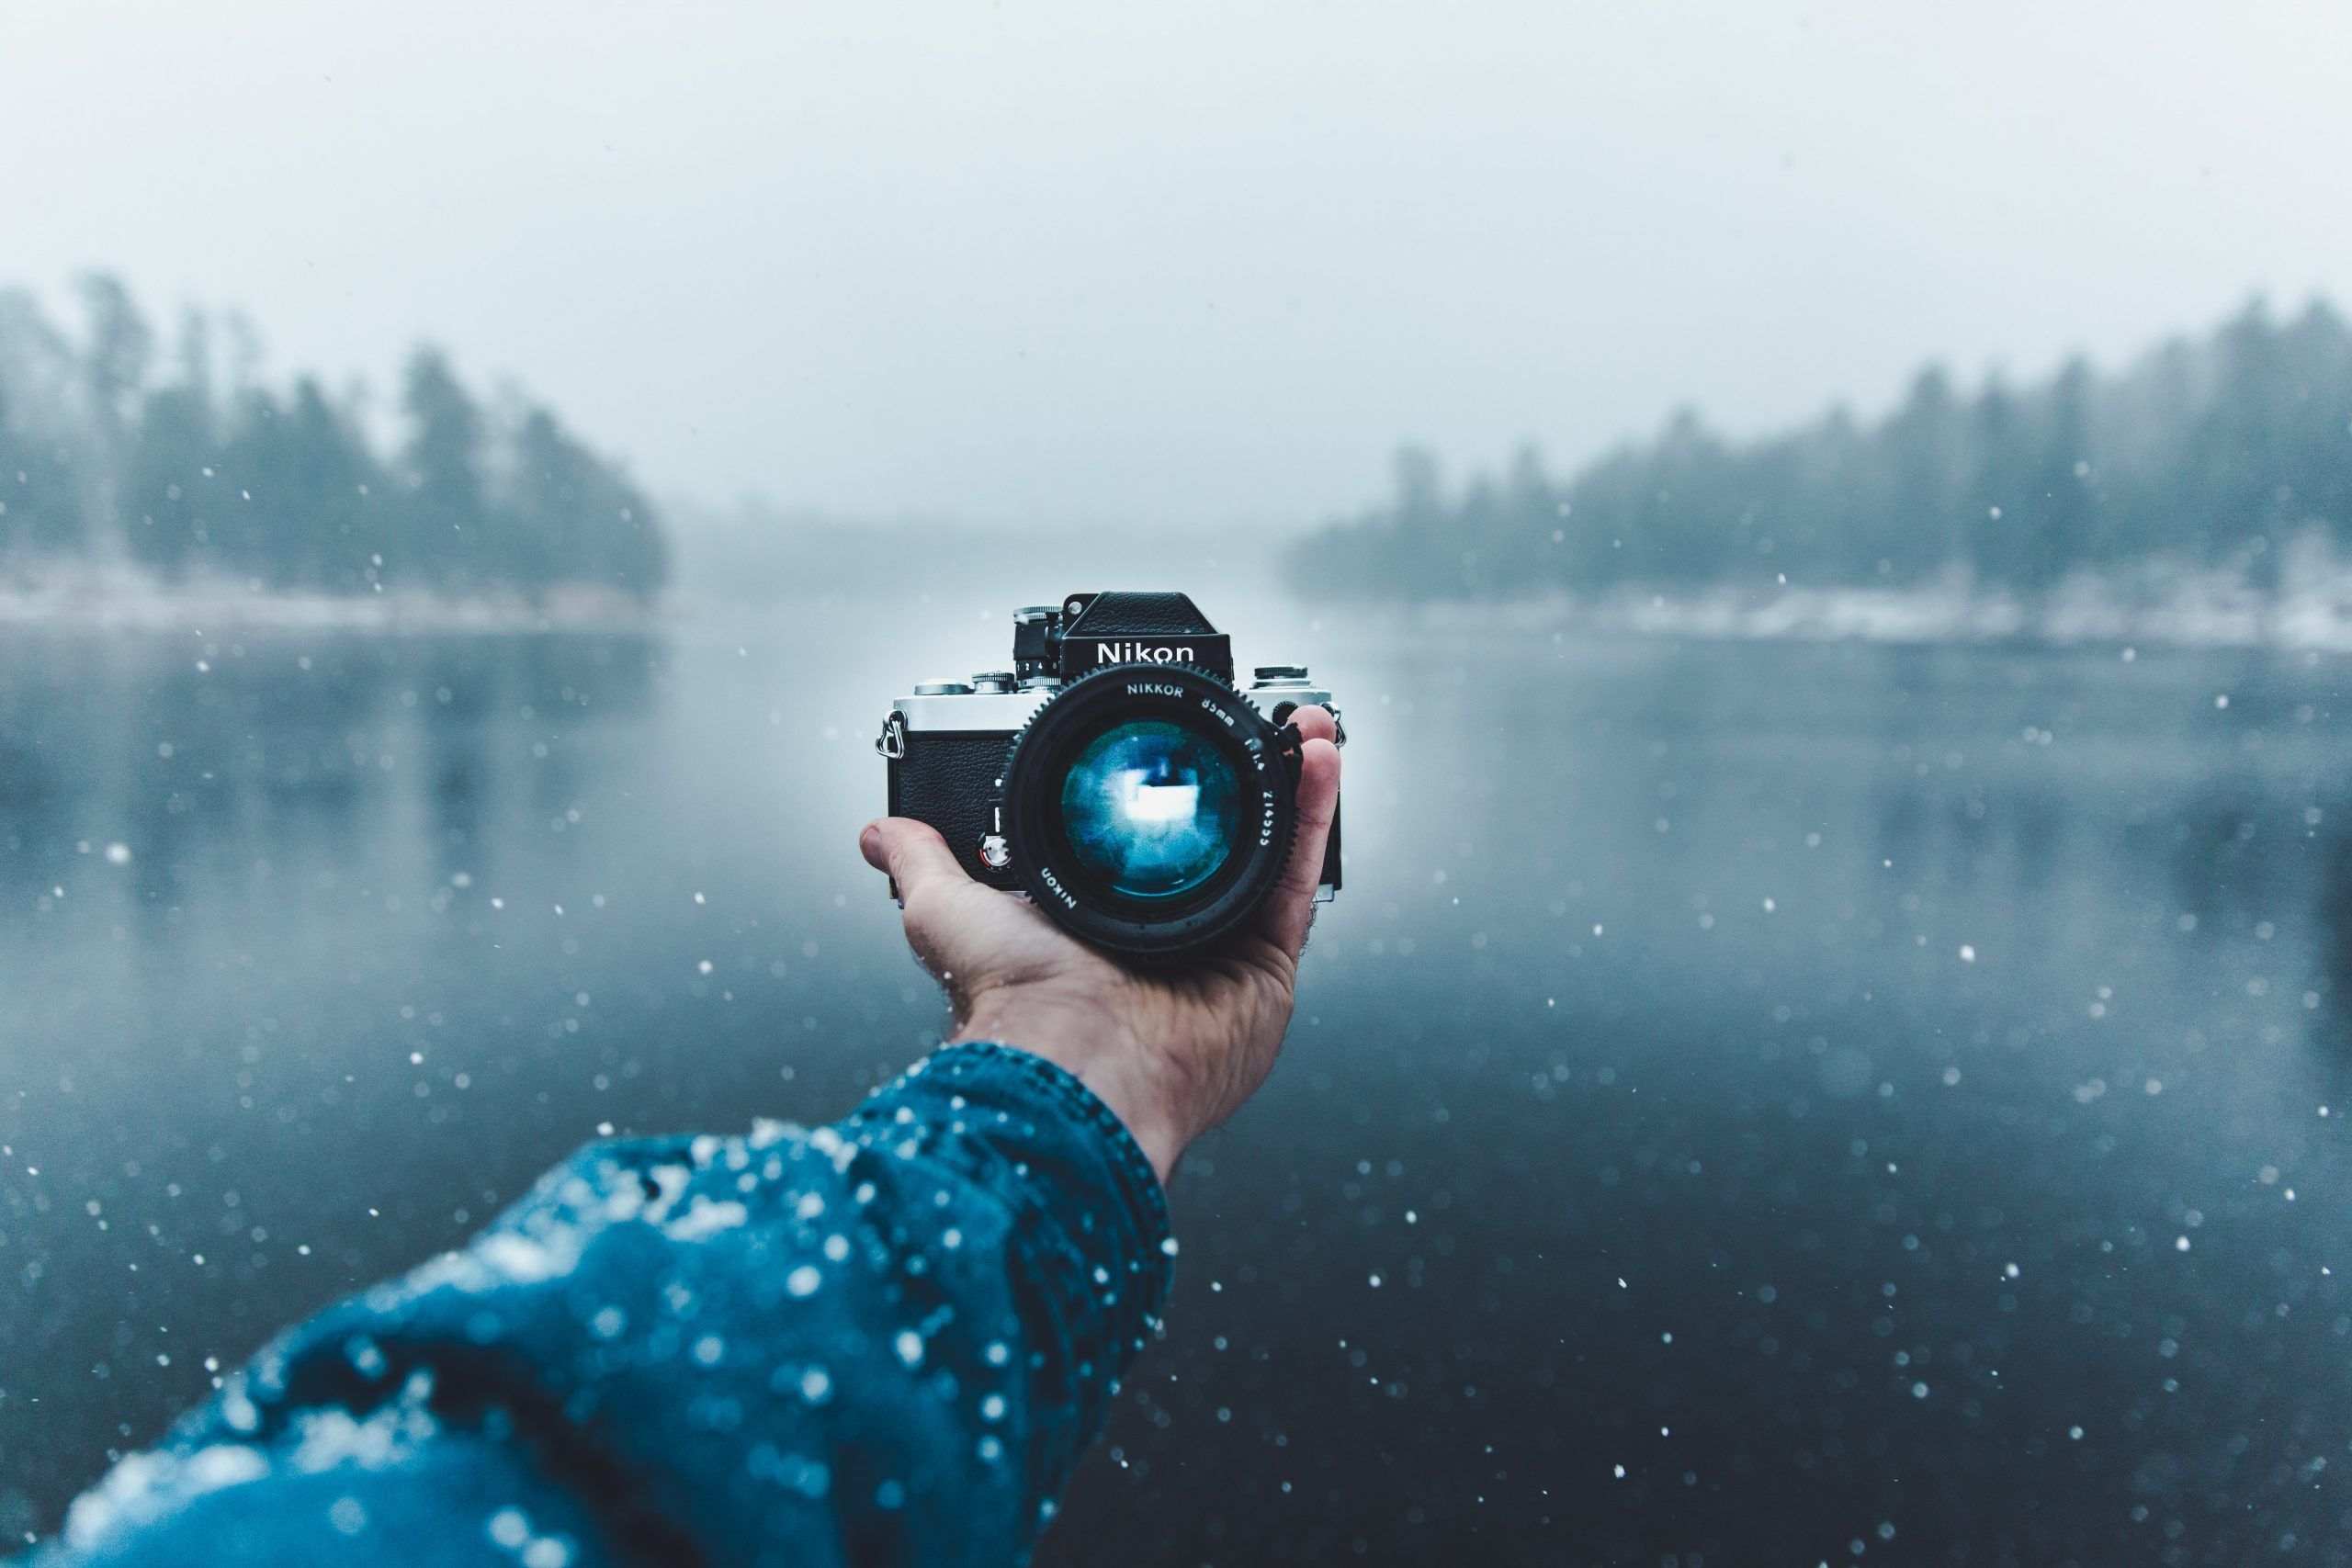
\includegraphics[width=0.8\textwidth]{esp32.jpg}
    \caption{Module vi điều khiển ESP32-WROOM-32.}
    \label{fig:esp32}
\end{figure}

\subsubsection{Cảm biến chuyển động quán tính (IMU)}
Cảm biến IMU (Inertial Measurement Unit) là thành phần cốt lõi, tích hợp các cảm biến đo chuyển động và tư thế. Một IMU như MPU6050 hoặc BNO055 bao gồm:

\begin{itemize}
    \item \textbf{Gia tốc kế:} Đo gia tốc tuyến tính trên ba trục (x, y, z), độ nhạy từ ±2g đến ±16g. Trong trường hợp té ngã, gia tốc kế ghi nhận đỉnh gia tốc bất thường (>3g trong 0.1--0.3 giây) \cite{xu2023}.
    \item \textbf{Con quay hồi chuyển:} Đo tốc độ góc trên ba trục (±250 đến ±2000 độ/giây), xác định sự thay đổi tư thế (ví dụ: từ đứng sang nằm ngang trong <1 giây) \cite{hussain2019}.
    \item \textbf{Từ kế (tùy chọn):} Cung cấp dữ liệu định hướng, tăng độ chính xác khi kết hợp với thuật toán Kalman Filter \cite{alarifi2021}.
\end{itemize}

Kết hợp dữ liệu từ gia tốc kế và con quay hồi chuyển qua thuật toán ngưỡng động hoặc học sâu (LSTM, CNN) đạt độ chính xác trên 94\% trên tập dữ liệu SisFall \cite{hussain2019}. MPU6050 (6 trục, I2C, 3.6 mA) là lựa chọn phổ biến nhờ chi phí thấp và hiệu năng ổn định \cite{iotproject2024}.

\begin{figure}[ht]
    \centering
    
\includegraphics[width=0.8\textwidth]{imu.png}
    \caption{Sơ đồ minh họa nguyên lý hoạt động của cảm biến IMU (MPU6050).}
    \label{fig:imu_working_principle}
\end{figure}

\subsubsection{Module định vị toàn cầu (GPS)}
Module GPS (như NEO-6M hoặc NEO-7M) cung cấp thông tin vị trí địa lý qua tín hiệu vệ tinh, hữu ích khi người dùng di chuyển ngoài phạm vi camera. Với độ chính xác 2.5--5 m, thời gian khóa vệ tinh <30 giây và giao tiếp UART/I2C, GPS hỗ trợ gửi tọa độ chính xác khi xảy ra sự cố, giảm thời gian phản ứng cứu hộ xuống dưới 5 phút \cite{ublox2023, xu2023}. Tuy nhiên, GPS tiêu tốn 20--40 mA và hiệu suất giảm trong môi trường đô thị hoặc trong nhà.

% Subsection for imaging and processing systems
\subsection{Hệ thống giám sát hình ảnh và máy chủ xử lý}

Hệ thống này thu thập và phân tích dữ liệu hình ảnh, cung cấp bối cảnh trực quan và xử lý thuật toán phức tạp.

\subsubsection{Thiết bị camera nhúng}
Camera nhúng ghi lại video thời gian thực để phân tích tư thế và chuyển động. Module \textbf{ESP32-CAM} (tích hợp ESP32-S và camera OV2640, độ phân giải 1600x1200) được chọn nhờ chi phí thấp (5--10 USD), hỗ trợ RTSP/HTTP streaming và xử lý sơ bộ hình ảnh (nén JPEG) \cite{esp32cam2023}. Hạn chế là chất lượng hình ảnh giảm trong điều kiện ánh sáng yếu (độ nhạy 1 lux) \cite{saraswat2024}. Camera RGB-D (như Kinect) cũng được sử dụng để tăng độ chính xác trong môi trường phức tạp \cite{liu2018}.

\begin{figure}[ht]
    \centering
    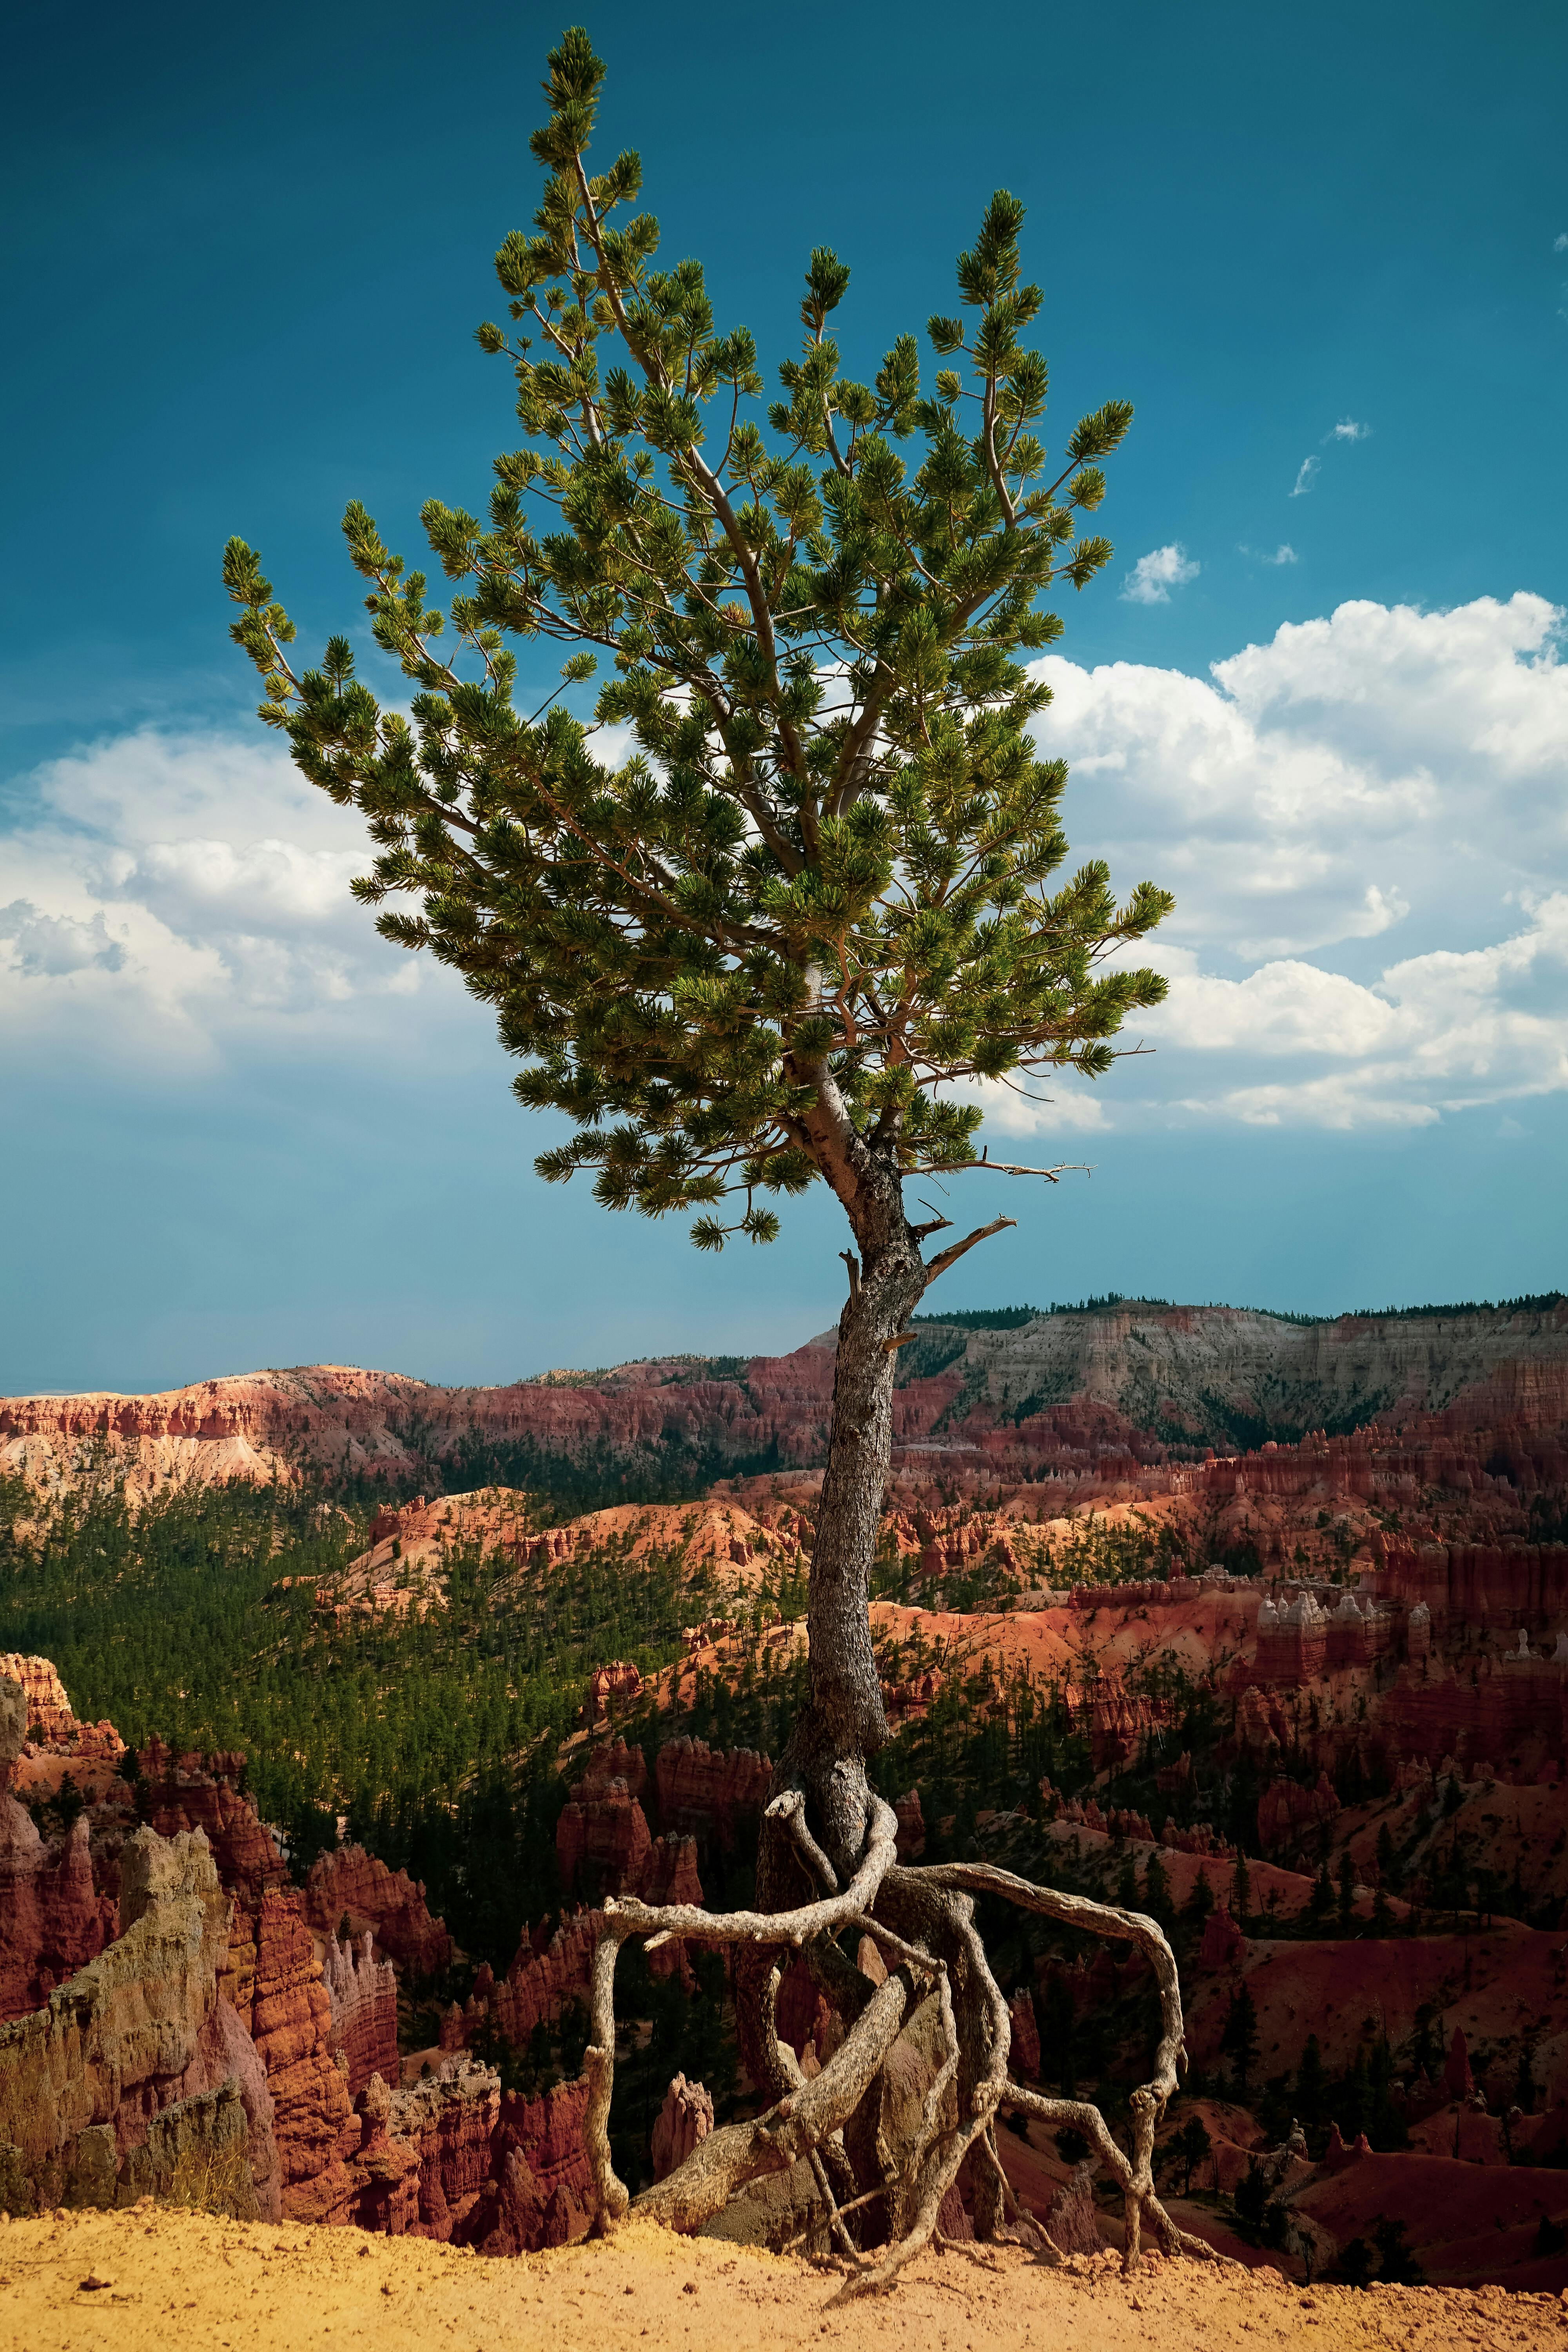
\includegraphics[width=0.8\textwidth]{camera_module.jpg}
    \caption{Module camera nhúng ESP32-CAM.}
    \label{fig:esp32_cam}
\end{figure}

\subsubsection{Máy chủ xử lý trung tâm}
Máy chủ trung tâm xử lý dữ liệu chuyên sâu, chạy trên Linux (Ubuntu 20.04) với GPU (NVIDIA RTX 3060, 12 GB VRAM) để triển khai các mô hình như YOLOv5, MediaPipe hoặc Transformer \cite{han2024, stylios2024}. Các thư viện bao gồm:

\begin{itemize}
    \item \textbf{OpenCV}: Xử lý hình ảnh, hỗ trợ phát hiện đối tượng và ước lượng tư thế.
    \item \textbf{TensorFlow/PyTorch}: Triển khai học sâu cho phân tích dữ liệu cảm biến và hình ảnh.
    \item \textbf{Numpy/Scipy}: Xử lý số liệu và sensor fusion.
\end{itemize}

Hệ thống sử dụng YOLOv5 và MediaPipe đạt mAP 98.6\% trong phát hiện té ngã, với độ trễ xử lý dưới 100 ms \cite{han2024, multimodal2024}. Máy chủ cung cấp API (RESTful/WebSocket) cho giám sát từ xa.

% Subsection for communication systems
\subsection{Hệ thống truyền thông di động và cố định}

Hệ thống truyền thông đảm bảo dữ liệu và cảnh báo được truyền tải nhanh chóng, đáng tin cậy trong các điều kiện mạng khác nhau.

\subsubsection{Module truyền thông di động (4G/LTE)}
Module 4G/LTE (như SIM800L hoặc SIM7600) cung cấp kết nối internet qua mạng di động, với tốc độ tải xuống 10--150 Mbps và độ trễ 20--50 ms \cite{simcom2023}. Điều này cho phép thiết bị hoạt động ở khu vực không có Wi-Fi, đảm bảo giám sát liên tục khi người dùng di chuyển ngoài trời. Ví dụ, tích hợp SIM800L vào hệ thống IMU cho phép gửi cảnh báo SMS và tọa độ GPS trong 2 giây sau khi phát hiện té ngã \cite{xu2023}. Hạn chế bao gồm chi phí thuê bao mạng và tiêu thụ năng lượng cao (100--500 mA).

\subsubsection{Nền tảng máy chủ truyền thông}
Máy chủ truyền thông điều phối các kênh liên lạc, đảm bảo cảnh báo kịp thời:

\begin{itemize}
    \item \textbf{Tổng đài SIP (Asterisk)}: Hỗ trợ gọi điện nội bộ qua mạng LAN, gửi cảnh báo thoại tự động với độ trễ dưới 1 giây trong môi trường cục bộ \cite{asterisk2023}.
    \item \textbf{Giao thức MQTT}: Giao thức nhẹ, phù hợp cho IoT, truyền dữ liệu cảm biến và cảnh báo với băng thông thấp (<10 KB/s) và độ tin cậy cao (QoS 2) \cite{iotproject2024}.
\end{itemize}

Sự kết hợp này tạo ra hệ thống truyền thông đa phương thức, với tính dự phòng cao (chuyển đổi giữa Wi-Fi, 4G và SIP khi một kênh thất bại) và độ trễ thấp, đáp ứng yêu cầu giám sát thời gian thực và cứu hộ nhanh chóng \cite{multimodal2024}.
